\begin{center}
\Huge
Polynomiel regression
\end{center}
\section*{Trivia om polynomier}
\stepcounter{section}

Før vi ser på polynomiel regression ser vi på lidt \textit{nice to know} omkring polynomier. Vi vil ikke bevise nogen af dem, men blot påstå, at det er tilfældet.
\begin{setn}
Et polynomium af grad $n$ har højst $n$ rødder
\end{setn}
\begin{setn}
Et polynomium af ulige grad har mindst en rod.
\end{setn}
Skal vi knytte lidt intuition til denne sætning, så kan vi notere os, at det største led går mod $\infty$, når $x\to \infty$. Tilsvarende går det største led mod $-\infty$, når $x \to \infty$. Idéen er så at alle andre led bliver domineret af det største led, så det for store nok $x$ kun er det største led der giver et signifikant bidrag. Derfor må polynomiet skære $x$-aksen et eller andet sted.
\begin{setn}
Har vi $n$ punkter, så er der et entydigt polynomium, der går gennem disse $n$ punkter af grad højst $n-1$. 
\end{setn}


\section*{Polynomiel regression}
Vi kan som sagt finde et entydigt andengradspolynomium gennem tre punkter. Har vi eksempelvis tre punkter $(1,2)$, $(2,4)$ og $(-2,1)$, så kan vi bestemme et andengradspolynomium, der går gennem disse punkter. Dette gøres i Maple med \texttt{PolyReg}, hvor vi skal give tre argumenter: En liste med x-værdier \texttt{X:=[-2,1,2]}, en liste med y-værdier \texttt{Y:=[1,2,4]} og en regressionsgrad \texttt{n := 2}. Regressionen laves så som
\begin{align*}
\texttt{PolyReg(X,Y,2)}
\end{align*}
Dette giver os så regressionslinjen på Fig. \ref{fig:polyreg}
\begin{figure}[H]
\centering
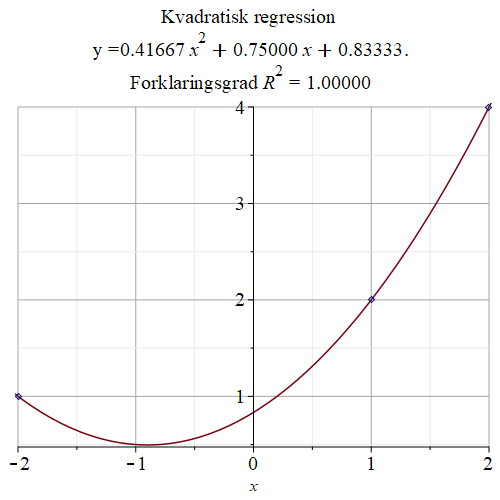
\includegraphics[width = 0.8\textwidth]{Billeder/polyreg.png}
\caption{Polynomiel regression lavet i Maple}
\label{fig:polyreg}
\end{figure}

\section*{Opgave 1}
Afgør, hvad det mindste og største antal rødder følgende polynomier har.
\begin{align*}
&1) \  x^2-x+1   &&2) \ x^7   \\
&3) \   x^6-10x+3  &&4) \ x^{1001}+2x+1   \\
&5) \   x^{5}-x^4+x^3+x^2-x+1  &&6) \ (x-1)^{1000}   \\
\end{align*}

\section*{Opgave 2}
Brug et CAS-værktøj til at bestemme rødderne til følgende polynomier:
\begin{align*}
&1) \ 7x^{10}-2x^3+1   &&2) \ 4x^4-2x+10   \\
&3) \ 6x^6-1   &&4) \  (x-1)^3 +(2x-10)^7  \\
\end{align*}

\section*{Opgave 3}
\begin{enumerate}[label=\roman*)]
\item Find det andengradspolynomium, der går gennem punkterne $(1,1)$, $(2,4)$ og $(3,9)$.
\item Find det tredjegradspolynomium, der går gennem punkterne $(-1,2)$, $(0,4)$, $(3,10)$ og $(4,-2)$.
\item Find det fjerdegradspolynomium, der går gennem punkterne $(-10,1)$, $(-4,10)$, $(6,2)$, $(2,5)$, og $(7,30)$.
\end{enumerate}

\section*{Opgave 4}
Et datasæt 
\begin{center}
\begin{tabular}{c|c|c|c|c|c|c}
0 & 1 & 2 & 3 & 4 & 5 & 6\\ \hline
2.13 & 9.09 & 6.40 & 32.43 & 45.29 & 59.73 & 90.14
\end{tabular}
\end{center}
er givet. Bestem det andengradspolynomium, der bedst passer på punkterne. 

\section*{Opgave 5}
Et datasæt
\begin{center}
\begin{tabular}{c|c|c|c|c|c|c}
-3 & -2 & -1 & 0 & 1 & 2 & 3\\ \hline
-21.30 & -2.22 & 7.33 & -0.64 & 2.33 & 7.88 & 27.94
\end{tabular}
\end{center}
er givet. Bestem det tredjegradspolynomium, der bedst passer på punkterne. 